\documentclass[a4paper,12pt]{ctexrep}

\usepackage{graphicx}
\usepackage{geometry}
\usepackage{fancyhdr}
\geometry{top=4.0cm,bottom=3.0cm,left=2.5cm,right=2.5cm}
\usepackage{array}
\usepackage[colorlinks,linkcolor=black]{hyperref}
\title{豆瓣图书需求分析报告}
\author{小组:9527小组}
\ctexset{
	section = {
		number = \arabic{section}.
	},
	subsection = {
		number={}
	}
}
\pagestyle{fancy}
\fancyhf{}
\fancyhead[C]{豆瓣图书需求分析报告}
\fancyfoot[C]{\thepage}

\begin{document}
	\maketitle
	\newpage
	\tableofcontents
	\thispagestyle{empty}
	\newpage
	\section{人员分工}
	\begin{center}
	\begin{tabular}{|p{3cm}<{\centering}|p{3cm}<{\centering}|p{3cm}<{\centering}|p{5cm}<{\centering}|}
		\hline
		班级&小组成员&职责&联系方式(邮箱)\\
		\hline
		软件1604班&冯钢果&项目经理&1481660657@qq.com\\
		\hline
		软件1604班&唐标&后台开发&2815383499@qq.com\\
		\hline
		软件1604班&郑佳浩&需求分析师&1295043714@qq.com\\
		\hline
	\end{tabular}
	\end{center}
	\subsection*{分工详细介绍}
	\par 冯钢果(项目经理):主要领导、监督项目开发过程,并参与项目的具体前台、后台实际开发,对服务器进行管理,主要任务开发小程序前端,包括部分后台开发,并对需求分析及相关文档撰写提供意见;
	\par 唐标(后台开发):主要任务涉及后台开发过程,包括数据库设计、运维及开发及服务器管理和相关程序接口设计;
	\par 郑佳浩(需求分析师):主要采集用户需求,并对用户需求进行分析,并在开发过程记录文档,最后体验和测试软件并提出相关完善意见。
	\section{项目概况}
	\begin{center}
		\begin{tabular}{|p{3cm}<{\centering}|p{12cm}|}
			\hline
			\textbf{项目名称}&豆瓣图书\\
			\hline
			\textbf{项目概况}&豆瓣图书是一款可以通过搜索图书关键字列出相关图书的小程序\\
			\hline
			\textbf{行业}&生活应用\\
			\hline
			\textbf{架构类型}&生活,小程序\\
			\hline
			\textbf{开发技术}&Wxml,Wxss,js,json数据解析\begin{description}
				\item[服务器] Tomcat 8.5
				\item [数据库] MySQL 8.0
				\item  [项目特点]HTTP协议
			\end{description}\\
			\hline
			\textbf{规模}&系统总体规模:0.75人月(3 * 0.25)\\
			\hline
			\textbf{项目开始时间}&\today --- 2019年6月28日\\
			\hline
			\textbf{项目地址}&\url{https://github.com/WillAlso/DoubanReading.git}\\
			\hline
		\end{tabular}
	\end{center}
	\section{功能介绍}
	\subsection*{系统用例图}
	\begin{center}
		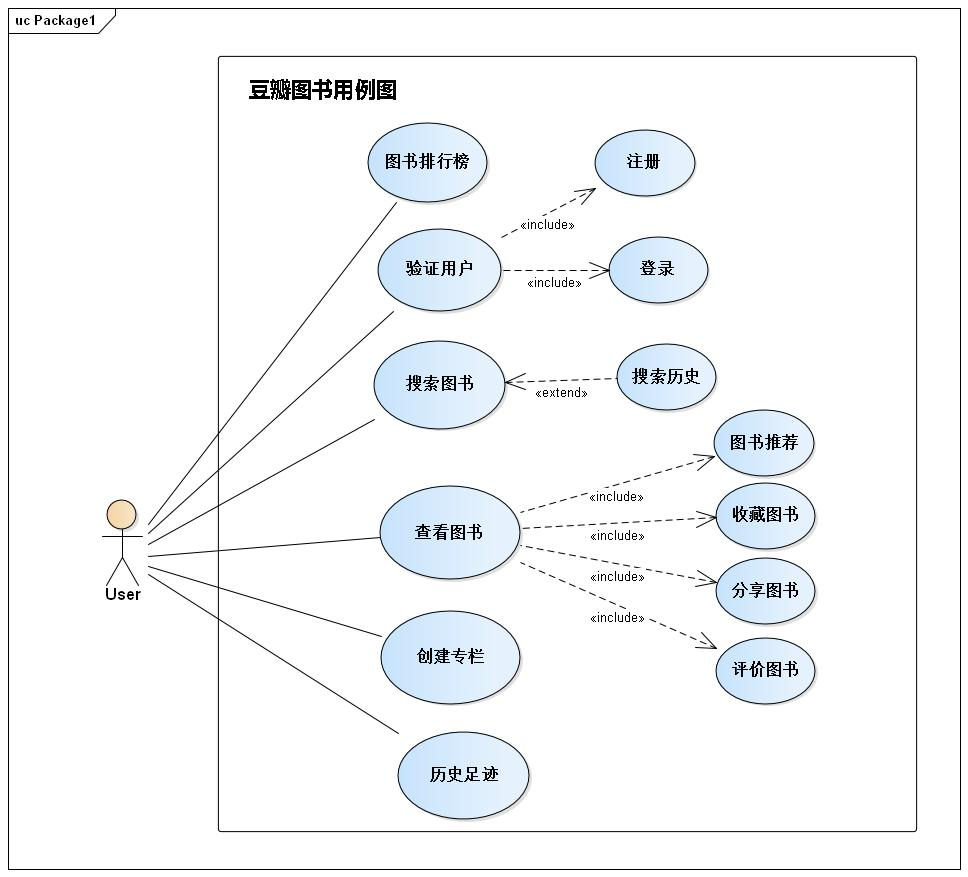
\includegraphics[width=15cm]{Package1.jpg}
	\end{center}
	\subsection*{用例描述}
	(豆瓣图书类似于豆瓣读书,但分为图书资源页和专栏文章页)
	\begin{enumerate}
		\item 验证用户
		\begin{itemize}
			\item 注册:微信用户需要填写相关信息,如用户名、用户喜爱图书类型标签、性别(非必填)、用户邮箱进行注册(必填项,可以发送验证码到用户邮箱进行验证);
			\item 登录:已经注册的微信用户直接微信验证登录,否则进行必须注册。
		\end{itemize}
		\item 图书排行榜
		\par 根据用户点击量、用户收藏量进行排行热门图书或者用户专栏文章。
		\item 搜索图书
		\par 用户可以根据图书作者名、图书名、图书ISBN号进行精确或者模糊搜索图书,
		也能够使用图书标签筛选图书。
		\item 查看图书
		\par 用户可以根据首页图书超链接、搜索出的链接,或者是能够直接导向图书资源页
		的超链接进行图书查看,可以查看图书作者、出版社、原作名、译者、出版年、页数、定价、装帧、ISBN、收藏数、评论数、图书标签、图书分类和图书评级的信息。
		\par 它包含的拓展功能:
		\begin{itemize}
			\item 图书推荐
			\par 用户能够推荐新书给平台,让平台尽快补充信息。
			\item 收藏图书
			\par 用户能够收藏自己喜欢的图书,并能加入购买愿望单。
			\item 分享图书
			\par 用户查看图书时,能够通过超链接分享到朋友圈、邮箱。
			\item 评价图书
			\par 用户能够评价、评星图书。
		\end{itemize}
		\item 创建专栏
		\par 用户能够自己创建专栏,来讨论自己关于某本书或是其他问题的看法,同时也可以设置权限:私有(相当于笔记)、公开(专栏文章)。
		\item 历史足迹
		\par 用户能够查看自己浏览过的书籍资源页。
		\item 保留接口
		\par 保留接口主要是指意愿实现,但可能由于时间问题不能实现的功能,但会尽力实现:
		\begin{itemize}
			\item 屏蔽评论敏感词和搜索敏感词;
			\item 用户能够互相关注;
			\item 用户能够查看部分图书购买资源及其他相关详细资源。
		\end{itemize}
	\end{enumerate}
	\section{技术介绍}
	\begin{enumerate}
		\item 基本技术
		\begin{itemize}
			\item 微信小程序编程及相关技术
			\par 微信小程序,简称小程序,英文名Mini Program,是一种不需要下载安装即可使用的应用,它实现了应用“触手可及”的梦想,用户扫一扫或搜一下即可打开应用。
			\par 需要学习微信小程序编程知识、Js脚本、微信小程序组件以及api,json解析数据
			相关知识。
			\item 服务器应用
			\par Tomcat,是一个免费的开放源代码的Web应用服务器,属于轻量级应用服务器,
			可以使用java来进行服务器编程,用来处理豆瓣图书用户请求,并返回处理数据。
			\item 数据库
			\par MySQL,是一种关系数据库管理系统,这里主要用来保存用户信息、图书信
			息,其中可以设计相关view、index提高数据库速度。
			\item 版本控制
			\par 使用git进行版本控制,项目地址为\\ 
			\url{https://github.com/WillAlso/DoubanReading.git}
		\end{itemize}
		\item 调用技术
		\begin{itemize}
			\item 服务器:阿里云轻量级服务器
			\par 阿里云提供的方便运维的云服务器,用来运行服务器应用Tomcat和数据库应用
			MySQL。
			\item 邮件推送:阿里云邮件推送服务
			\par 注册用户时,可能需要发送邮件验证码,使用阿里云提供的免费邮件推送服务进行推送验证码,可以查看阿里云提供的详细邮件推送API进行调用,这里的调用可以是用户通过get/post方法请求Tomcat服务器,服务器端反馈调用,并在服务器进行验证码验证。
		\end{itemize}
	\end{enumerate}
\end{document}